\documentclass[11pt]{article}
\usepackage[utf8]{inputenc}
\usepackage{amsmath, amssymb, amsthm}
\usepackage{graphicx}
\usepackage{hyperref}
\usepackage{geometry}
\usepackage{float}
\geometry{a4paper, margin=1in}

\title{\textbf{Project 2: Bayesian Logistic Regression for Binary Classification with Numerical Integration \& Monte Carlo}}
\author{LAN, Tianwei \\ ID: 21230969}
\date{\today}

\begin{document}

\maketitle

\section{Part 1: 1D Rejection to Sample Normal Distributions}

To sample the standard normal distribution $\mathcal{N}(w|0, 1) = \frac{1}{\sqrt{2\pi}} e^{-w^2/2}$ using the rejection method, we use the unnormalized Laplace distribution $f(w) = A e^{-\lambda|w|}$ (where $\lambda > 0$ and $-\infty < w < \infty$) as the comparison function.

\subsection{(a) Condition for Valid Comparison Function}

For $f(w)$ to be a valid comparison function, it must satisfy $f(w) \ge \mathcal{N}(w|0, 1)$ for all $w$. Thus, we require:
\begin{align*}
A e^{-\lambda|w|} &\ge \frac{1}{\sqrt{2\pi}} e^{-w^2/2} \\
A &\ge \frac{1}{\sqrt{2\pi}} e^{-w^2/2 + \lambda|w|}
\end{align*}
To find the lower bound for $A$, we need to find the maximum value of the exponent $-w^2/2 + \lambda|w|$. Let $g(x) = -x^2/2 + \lambda x$ for $x \ge 0$ (where $x = |w|$). Taking the derivative and setting it to zero gives:
\begin{align*}
g'(x) &= -x + \lambda = 0 \implies x = \lambda
\end{align*}
The maximum value of the exponent is $g(\lambda) = -\lambda^2/2 + \lambda^2 = \lambda^2/2$. 
Therefore, for the inequality to hold for all $w$, $A$ must satisfy:
\begin{equation}
A \ge \frac{1}{\sqrt{2\pi}} e^{\lambda^2/2}
\end{equation}

\subsection{(b) Theoretical Acceptance Rate}

The theoretical acceptance rate is the ratio of the area under the target distribution to the area under the comparison function $f(w)$. The area under the target standard normal distribution is 1. The area under $f(w)$ is:
\begin{align*}
\int_{-\infty}^{\infty} A e^{-\lambda|w|} dw &= 2 \int_{0}^{\infty} A e^{-\lambda w} dw \\
&= 2A \left[ -\frac{1}{\lambda} e^{-\lambda w} \right]_0^\infty \\
&= \frac{2A}{\lambda}
\end{align*}
Thus, the theoretical acceptance rate is:
\begin{equation}
\text{Acceptance Rate} = \frac{1}{\int_{-\infty}^{\infty} f(w) dw} = \frac{\lambda}{2A}
\end{equation}

\subsection{(c) Optimal Choice of Comparison Function}

To maximize the acceptance rate, we need to maximize $\frac{\lambda}{2A}$, which is equivalent to minimizing $\frac{A}{\lambda}$. Using the minimal valid $A(\lambda) = \frac{1}{\sqrt{2\pi}} e^{\lambda^2/2}$, we want to minimize:
\begin{equation*}
h(\lambda) = \frac{e^{\lambda^2/2}}{\sqrt{2\pi}\lambda}
\end{equation*}
Taking the derivative with respect to $\lambda$ and setting it to zero:
\begin{align*}
h'(\lambda) &= \frac{1}{\sqrt{2\pi}} \frac{\lambda e^{\lambda^2/2} \cdot \lambda - e^{\lambda^2/2} \cdot 1}{\lambda^2} \\
&= \frac{e^{\lambda^2/2}}{\sqrt{2\pi}\lambda^2} (\lambda^2 - 1) = 0
\end{align*}
Since $\lambda > 0$, we have $\lambda = 1$. Substituting $\lambda = 1$ back to find $A$:
\begin{equation*}
A = \frac{1}{\sqrt{2\pi}} e^{1/2} = \sqrt{\frac{e}{2\pi}}
\end{equation*}
Therefore, the optimal choice for the comparison function is:
\begin{equation}
f(w) = \sqrt{\frac{e}{2\pi}} e^{-|w|}
\end{equation}
The optimal acceptance rate with this choice is:
\begin{equation}
\text{Optimal Acceptance Rate} = \frac{\lambda}{2A} = \frac{1}{2 \sqrt{e/(2\pi)}} = \sqrt{\frac{\pi}{2e}} \approx 0.7602
\end{equation}

\subsection{(d), (e) \& (f) Code Implementation and Simulation Results}

Using the optimal comparison function, we generated 100,000 samples of $\mathcal{N}(0, 1)$ via rejection sampling.
The theoretical acceptance rate is approximately $0.7602$, and the actual acceptance rate from our Python simulation was exactly $0.7599$, verifying our theoretical predictions. The histogram of the generated samples aligns perfectly with the theoretical Gaussian curve (Figure \ref{fig:part1}).

To sample a general normal distribution $\mathcal{N}(\mu, \sigma^2)$, we can generate $Z \sim \mathcal{N}(0, 1)$ using the rejection method above, and apply the transformation $X = \mu + \sigma Z$. We tested this by generating 100,000 samples of $\mathcal{N}(5.0, 2.0^2)$. The sample mean was $4.9907$ and the sample variance was $3.9808$, matching the expected values closely.

\begin{figure}[H]
    \centering
    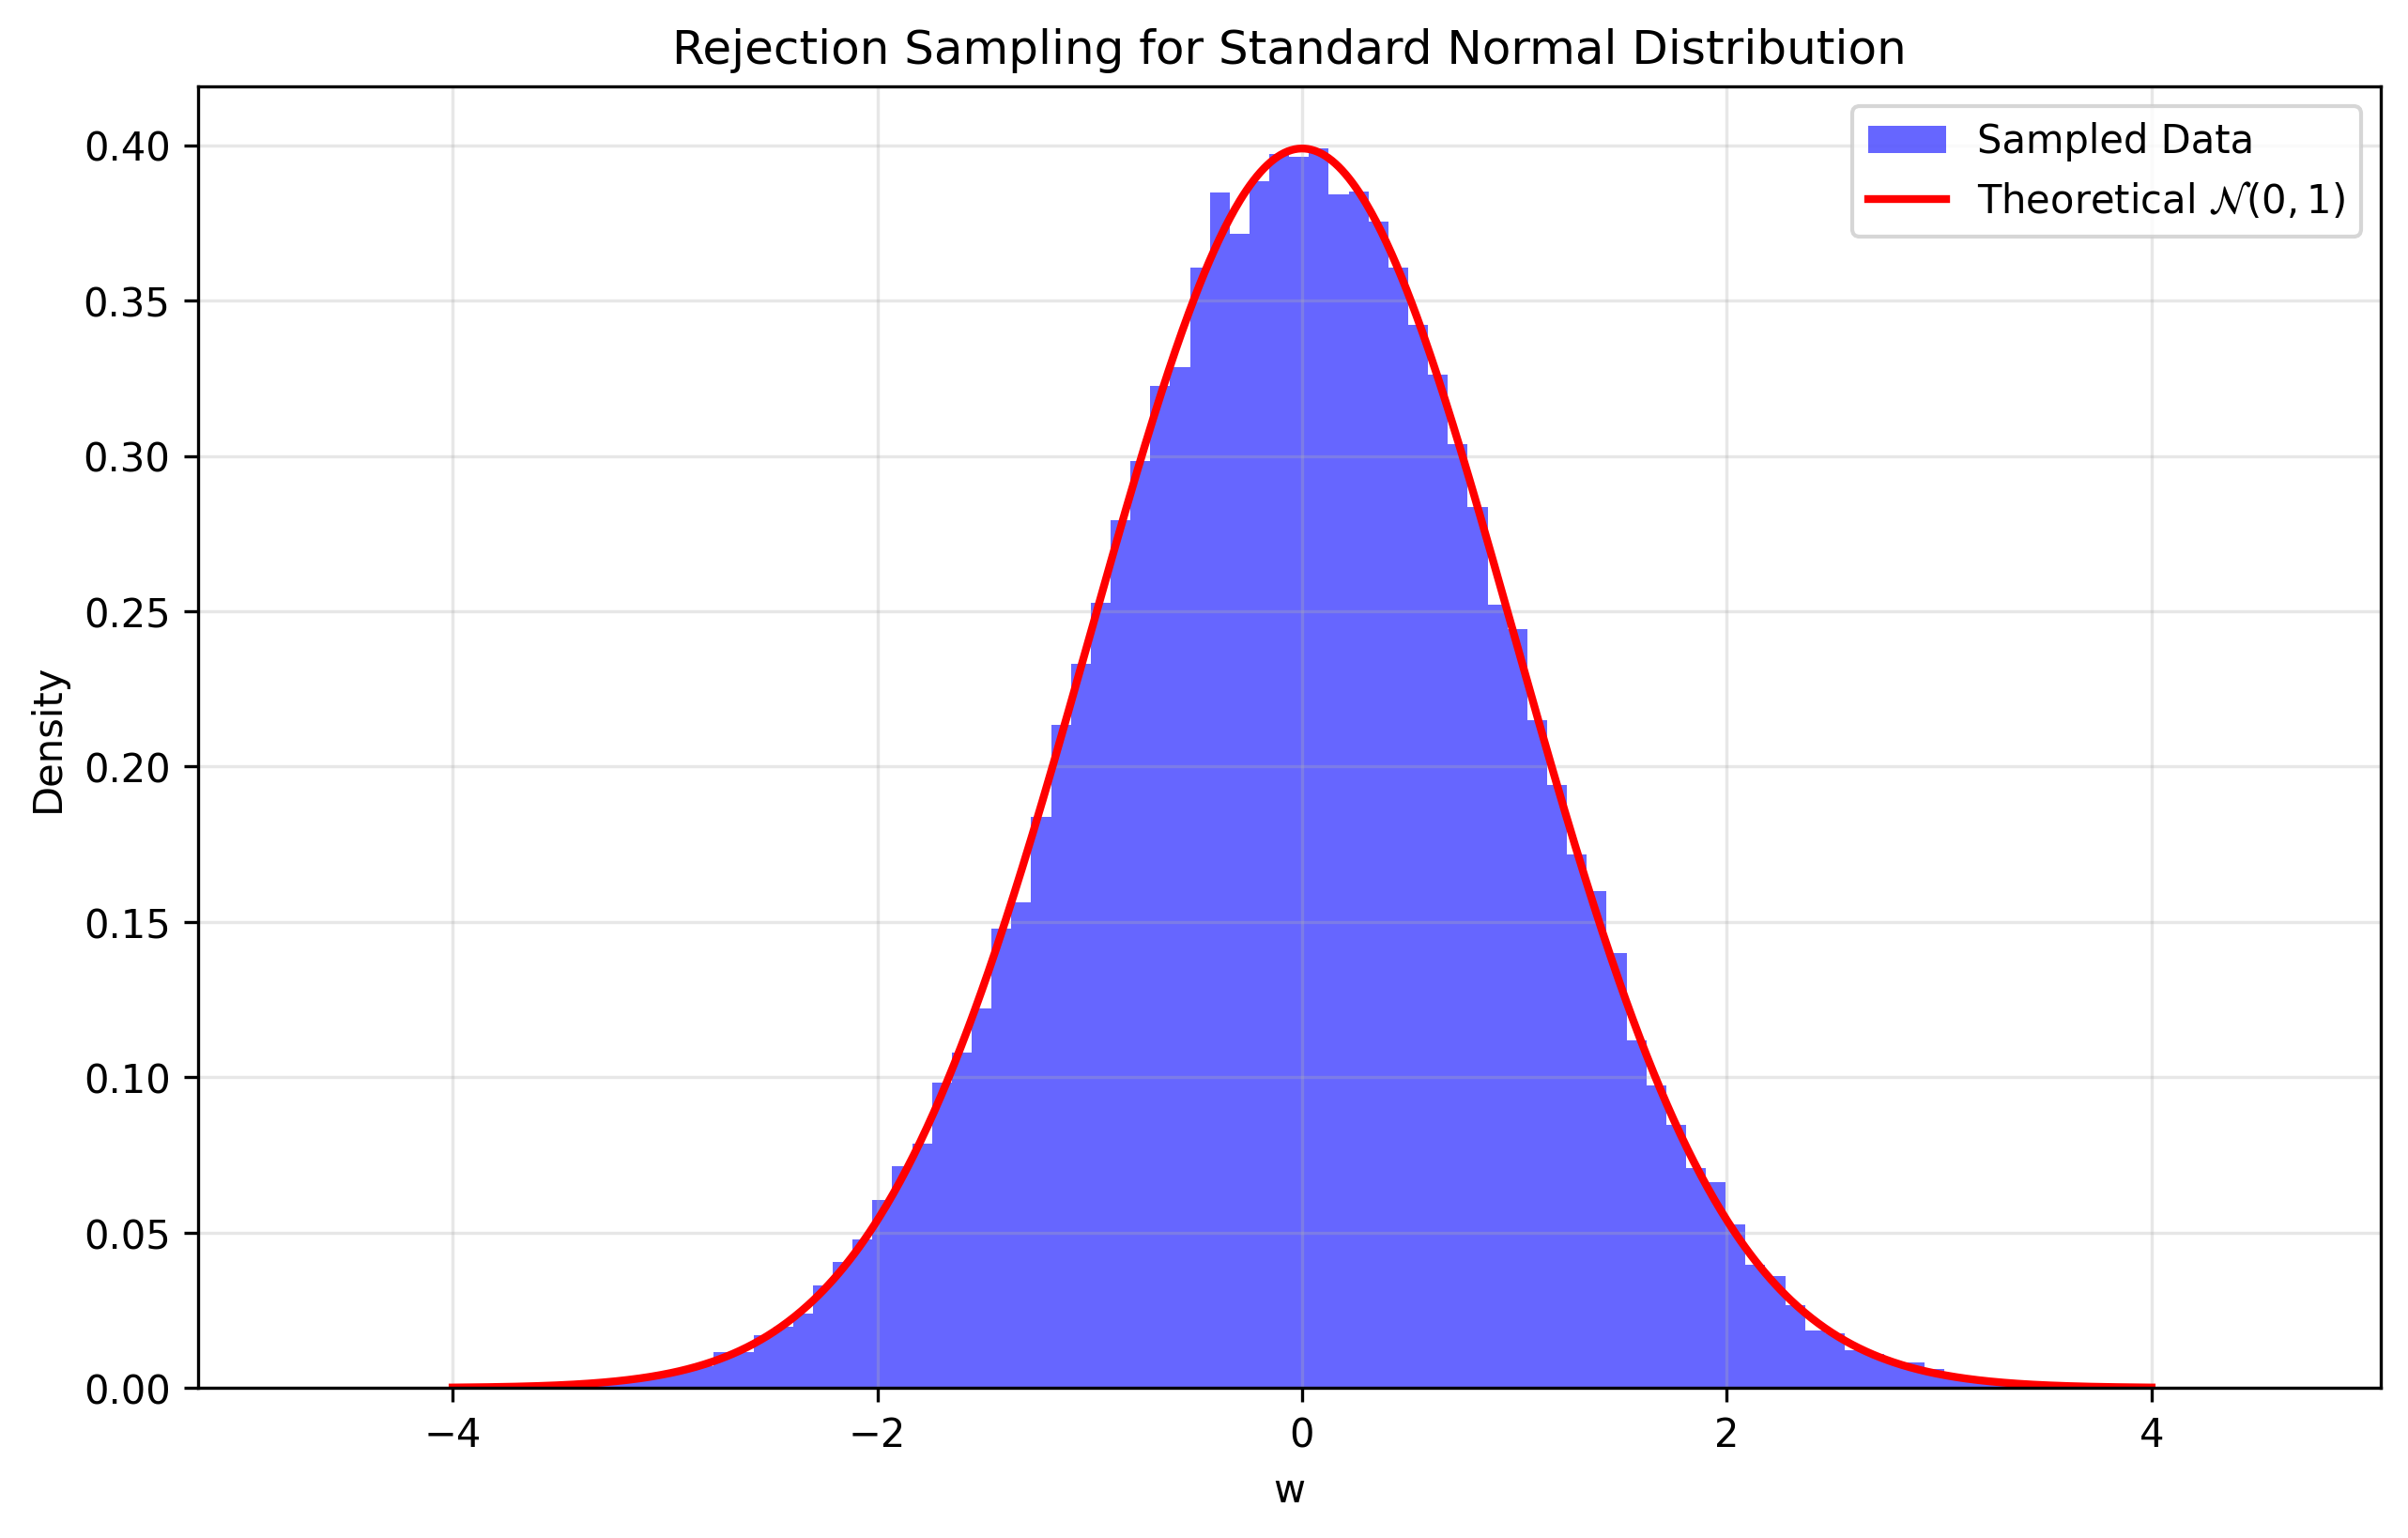
\includegraphics[width=0.7\textwidth]{part1_standard_normal.png}
    \caption{Rejection Sampling for Standard Normal Distribution}
    \label{fig:part1}
\end{figure}

\section{Part 2: Numerical Integration for Marginal Likelihood}

We generated a dataset of size $N=500$ with true weights $w_{true} = [-1, 1]^T$, $x_i \sim \mathcal{N}(1, 1)$, and added noise $\epsilon_i \sim \mathcal{N}(0, 4)$ (standard deviation $\sigma = 2$). 

\subsection{(b) \& (c) 1D Numerical Integration}

By fixing $w_0 = -1$, the marginal likelihood is a 1D integral over $w_1$. Due to the fast decay of the Gaussian prior, we transformed the improper integral to a finite interval $[-6, 6]$. We evaluated it using the Trapezoidal Rule and Romberg Integration, both with a relative tolerance of $10^{-6}$.

\begin{table}[H]
    \centering
    \begin{tabular}{|c|c|c|c|}
    \hline
    \textbf{Method} & \textbf{Integral Value} & \textbf{Estimated Error} & \textbf{Evaluations} \\
    \hline
    Trapezoidal Rule & $1.775465 \times 10^{-144}$ & $3.603833 \times 10^{-159}$ & 513 \\
    Romberg Integration & $1.769139 \times 10^{-144}$ & $1.399682 \times 10^{-150}$ & 257 \\
    \hline
    \end{tabular}
    \caption{1D Integration Results for Marginal Likelihood ($w_0 = -1$)}
\end{table}

Both methods yield highly consistent integral values, but Romberg integration is significantly more efficient, requiring half the number of integrand evaluations compared to the Trapezoidal rule to reach the same tolerance.

\subsection{(d) \& (e) 2D Numerical Integration}

Next, we evaluated the marginal likelihood by integrating out both $w_0$ and $w_1$.
We compared the 2D Simpson's rule over $[-6, 6] \times [-6, 6]$ (adaptive subdivision) and Crude Monte Carlo integration (sampling directly from the Gaussian prior $w \sim \mathcal{N}(0, I)$ with $1,000,000$ samples).

\begin{table}[H]
    \centering
    \begin{tabular}{|c|c|c|c|}
    \hline
    \textbf{Method} & \textbf{Integral Value} & \textbf{Estimated Error} & \textbf{Notes} \\
    \hline
    2D Simpson's Rule & $1.447376 \times 10^{-143}$ & $8.872012 \times 10^{-149}$ & 137,766 Evaluations \\
    Crude Monte Carlo & $1.442672 \times 10^{-143}$ & $1.282288 \times 10^{-145}$ & $10^6$ Samples \\
    \hline
    \end{tabular}
    \caption{2D Integration Results for Marginal Likelihood}
\end{table}

The Crude Monte Carlo estimation is reasonably close to the Simpson's rule result, but its standard error is relatively large ($1.28 \times 10^{-145}$) compared to the deterministic quadrature method, despite taking $10^6$ samples. This motivates the need for variance reduction techniques like Importance Sampling.

\section{Part 3: MCMC, Simulated Annealing, and Importance Sampling}

\subsection{(a) Metropolis Algorithm}

To sample from the posterior $p(w|D) \propto p(D|w)p(w)$, we implemented the Metropolis-Hastings algorithm. Using a symmetric Gaussian proposal $w' \sim \mathcal{N}(w, \sigma_p^2 I)$ with $\sigma_p = 0.17$, we achieved an acceptance rate of $30.80\%$, which is close to the requested target of approximately $30\%$. After discarding the first 1000 burn-in samples, we computed the sample covariance matrix:

\begin{equation*}
\Sigma_{\text{sample}} = \begin{bmatrix}
0.01905 & -0.01058 \\
-0.01058 & 0.01068
\end{bmatrix}
\end{equation*}

The sampled data points overlaying the theoretical posterior contour plot are shown in Figure \ref{fig:part3}.

\begin{figure}[H]
    \centering
    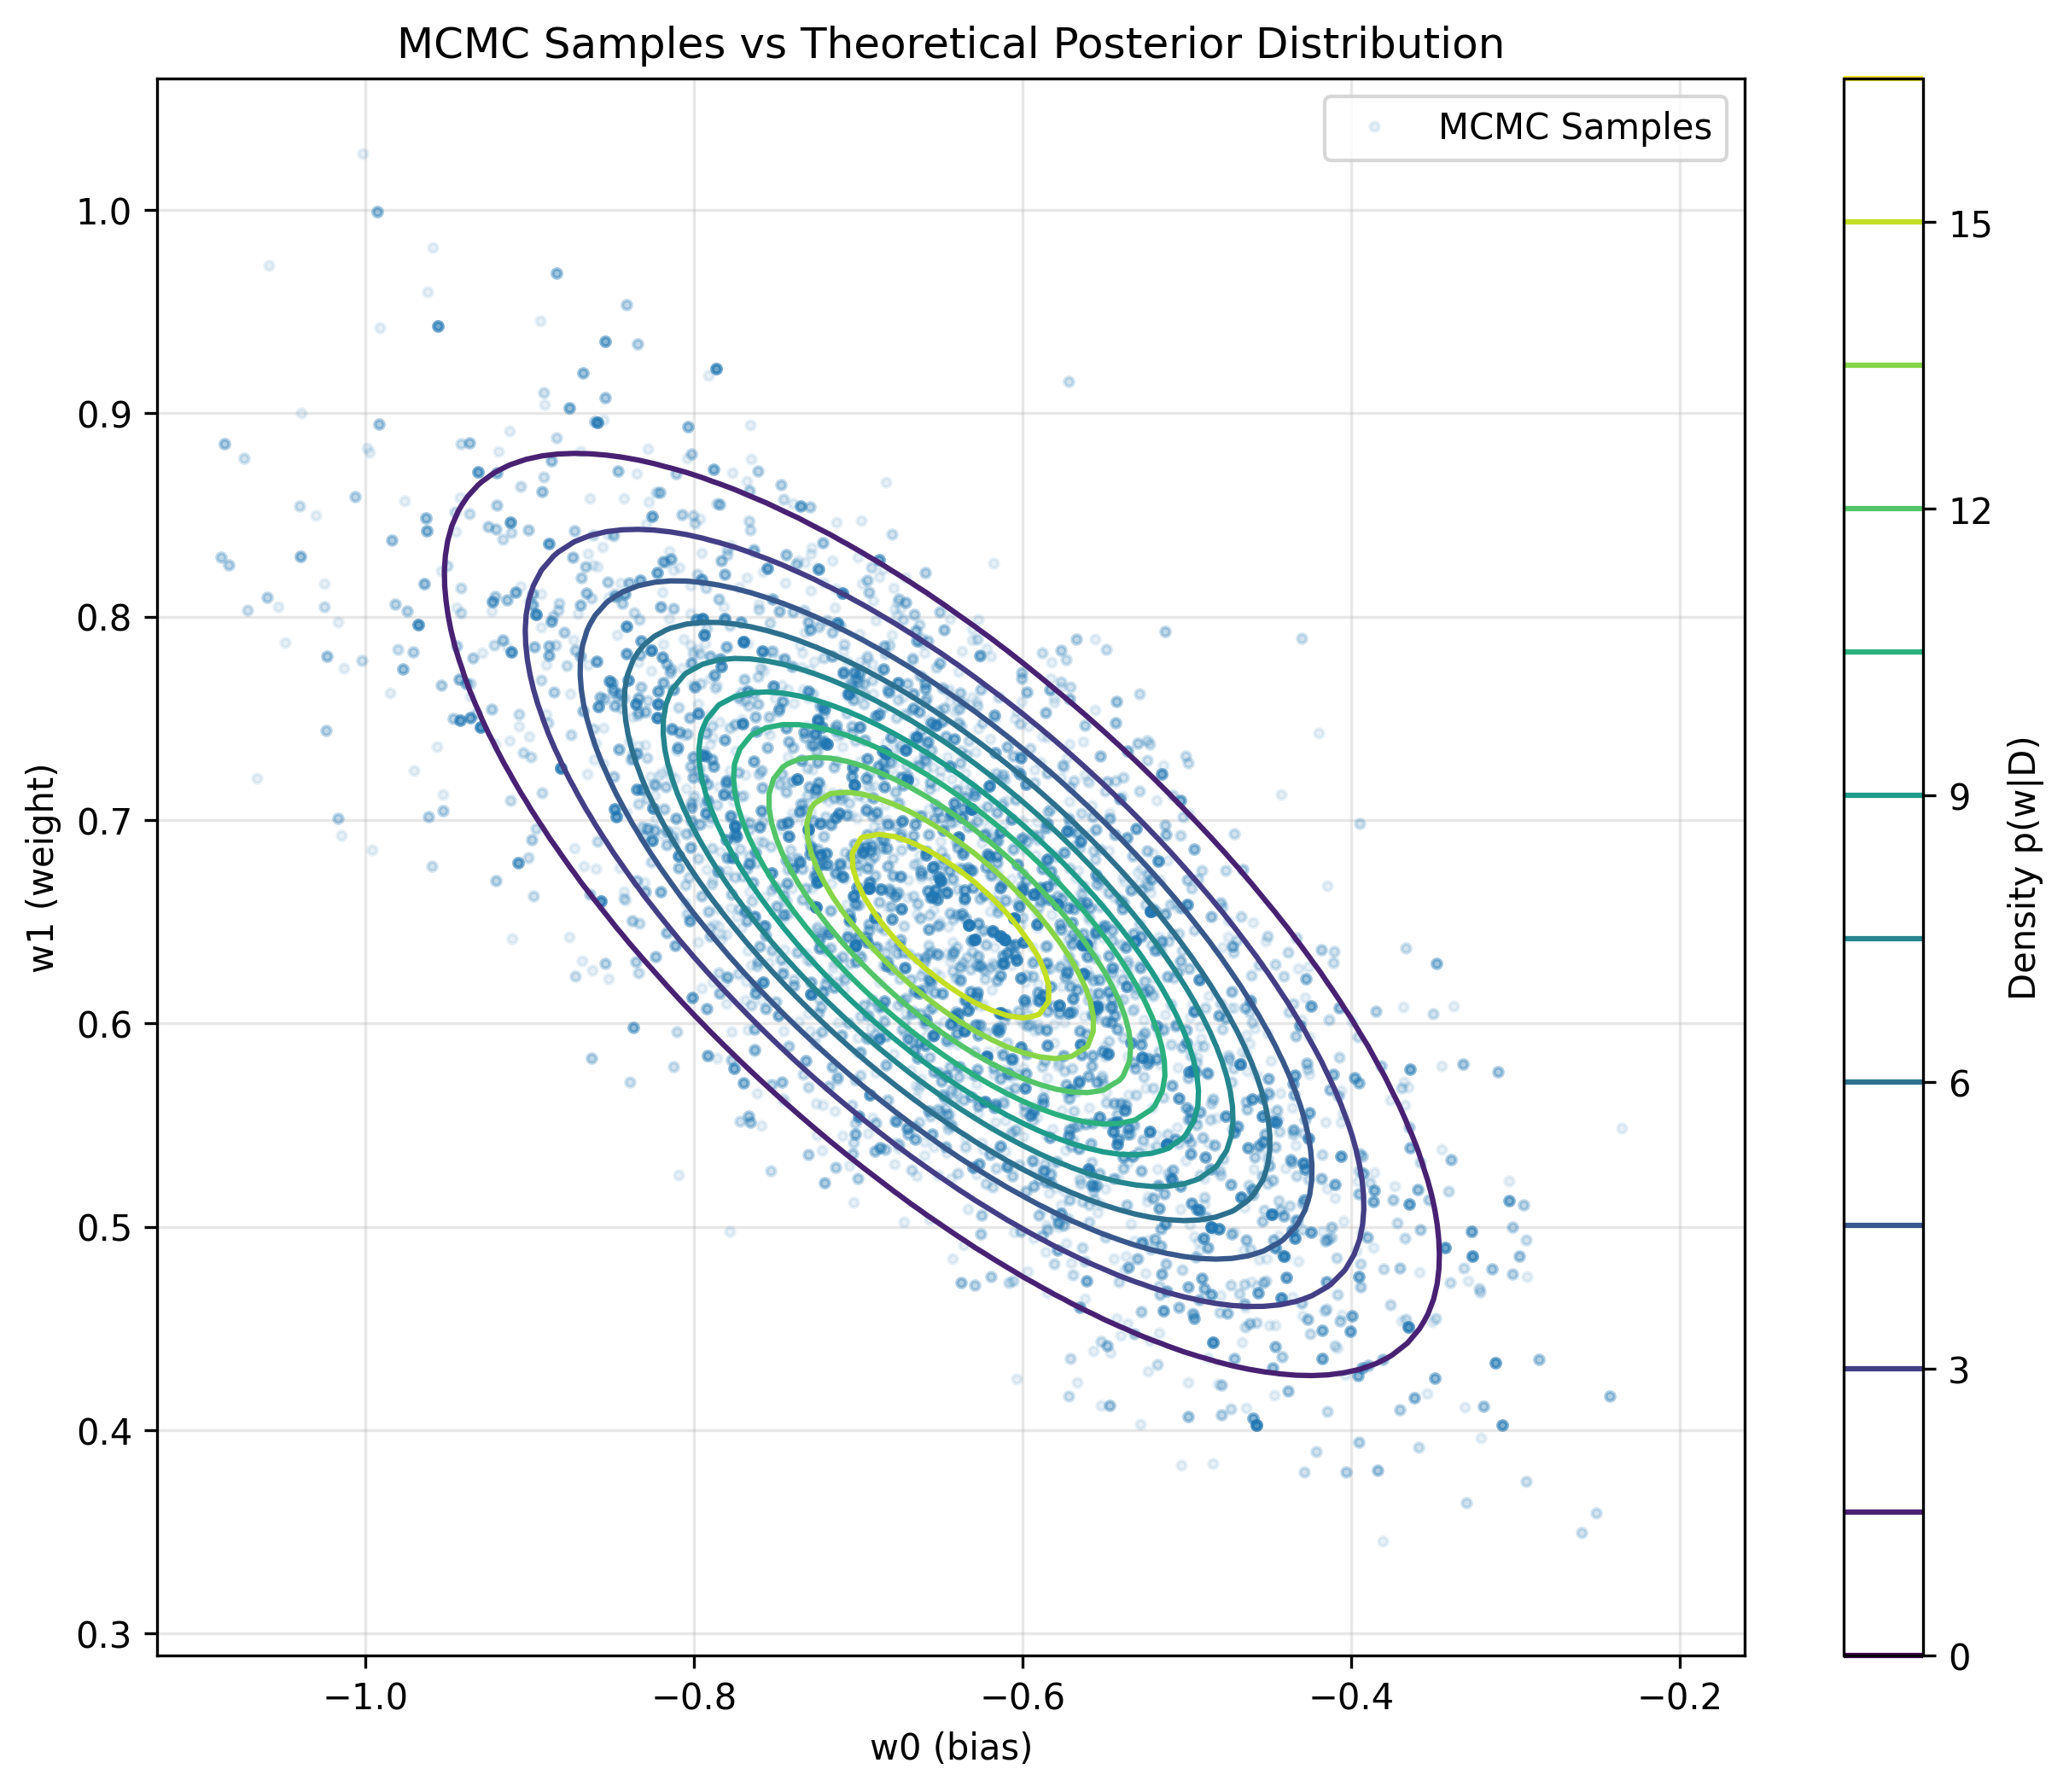
\includegraphics[width=0.7\textwidth]{part3_metropolis.png}
    \caption{MCMC Samples (dots) vs Theoretical Posterior Contours}
    \label{fig:part3}
\end{figure}

\subsection{(b) Simulated Annealing for MAP}

We aim to find the maximum a posteriori (MAP) estimate:
\begin{equation*}
w_{\text{MAP}} = \arg\max_{w} p(w|D)
\end{equation*}
Using Simulated Annealing to minimize the energy function $E(w) = -\log[p(D|w)p(w)]$, the optimizer successfully found the MAP estimate:
\begin{equation*}
w_{\text{MAP}} \approx [-0.64347, \;\; 0.64663]^T
\end{equation*}
The log-posterior at this point is $-326.0960$.

\subsection{(c) Importance Sampling (Variance Reduction)}

To efficiently compute the marginal likelihood, we used Importance Sampling. The proposal distribution $q(w)$ was chosen to be a Gaussian centered at $w_{\text{MAP}}$, with covariance set to the sample covariance matrix $\Sigma_{\text{sample}}$ computed in Part 3(a). Using $1,000,000$ samples from this tailored $q(w)$, the marginal likelihood was evaluated as:

\begin{itemize}
    \item \textbf{Integral Value (IS):} $1.447251 \times 10^{-143}$
    \item \textbf{Standard Error (IS):} $1.015534 \times 10^{-147}$ (Relative error $\approx 0.0070\%$)
\end{itemize}

\textbf{Conclusion:} The integral result closely matches the 2D Simpson's rule obtained in Part 2(d) ($1.447376 \times 10^{-143}$). Most importantly, compared to the Crude Monte Carlo standard error of $1.28 \times 10^{-145}$, the Importance Sampling standard error ($1.02 \times 10^{-147}$) is smaller by two orders of magnitude. This clearly demonstrates the massive variance reduction achieved by choosing a proposal distribution $q(w)$ that closely mimics the actual posterior.

\end{document}